\documentclass[a4paper]{article}
\usepackage[a4paper,left=3cm,right=2cm,top=2.5cm,bottom=2.5cm]{geometry}
\usepackage[utf8]{inputenc}
\usepackage{amsmath}
\usepackage{algorithm}
\floatname{algorithm}{Algorisme} % Cambia "Algorithm" por "Algorisme"

\usepackage{algpseudocode}
\usepackage{hyperref}
\usepackage{graphicx}
\usepackage{float}
\usepackage{array}

\graphicspath{ {./images/} }

\title{\textbf{Intel·ligència Artificial:\\
		Pràctica de Cerca Local}}
\author{\emph{Guillem Cabré, Carla Cordero, Hannah Röber}}
\date{Curs 2024-25, Quatrimestre de tardor}

\renewcommand*\contentsname{Continguts}
\renewcommand{\figurename}{Figura}

\begin{document}
	
	\begin{titlepage}
		\clearpage\maketitle
		\thispagestyle{empty}
	\end{titlepage}
	
	\tableofcontents
	\clearpage
	
	\section{Part Descriptiva}
	
	\subsection{Descripció del problema}
	
	La companyia fictícia \emph{Ázamon} ha d'optimitzar els seus enviaments diaris de $n$ paquets a una ciutat, considerant diversos factors. Cada paquet té un pes $w_i$ i una prioritat $p_i$, que defineix el termini màxim per ser entregat. L'empresa rep ofertes diàries de diverses companyies de transport, i el repte és trobar la millor manera de distribuir els paquets entre aquestes ofertes, minimitzant els costos i maximitzant la satisfacció dels clients. \\
	
	Els costos inclouen tant el transport, amb preus per quilogram que varien segons l'empresa, com l'emmagatzematge dels paquets que no es recullen immediatament. La felicitat dels clients augmenta si els paquets arriben abans de la data límit prevista. Per tant, cal equilibrar l'eficiència en costos amb la rapidesa en el lliurament per maximitzar la satisfacció del client. \\
	
	\subsection{Elements del problema}
	
	Cada paquet té un pes $w_i \in \{0.5, 1.0, 1.5, ..., 10.0\}$ kg i una prioritat $p_i \in \{1, 2, 3\}$, que defineix el termini d'entrega: un dia per $p_i = 1$, entre 2 i 3 dies per $p_i = 2$, i entre 4 i 5 dies per $p_i = 3$. Cadascuna d'aquestes prioritats té un cost diferent, $p_i = 1$ val 5 euros, $p_i = 2$ val 3 euros i $p_i = 3$ val 1.5 euros. \\
	
	Les empreses de transport ofereixen cada dia $m$ opcions amb una capacitat màxima $C_j \in \{5, 10, 15, ..., 50\}$ kg, un preu per quilogram transportat $c_j$, i un temps d'entrega $t_j \in \{1, 2, 3, 4, 5\}$ dies. A més, si els paquets no es recullen immediatament, cal assumir un cost d'emmagatzematge de 0.25 euros per quilogram i dia. Els clients es mostren més satisfets amb entregues anticipades, la qual cosa augmenta proporcionalment als dies d'antelació. \\

	\subsection{Definició solució}

	Una solució segons el problema que se'ns ha descrit és una assignació dels paquets a les ofertes de transport del dia apropiades amb les restriccions que la suma dels pesos dels paquets assignats a una oferta no poden superar la seva capacitat màxima i que tots els paquets arribin dins del termini d'entrega que depén de la seva prioritat. \\

	Formalment, si tenim $n$ paquets i $m$ ofertes de transport, una solució seria una tupla que associa cada paquet $p_i$ a una oferta $o_j$, tal que $1 \leq i \leq n$ i $1 \leq j \leq m$, amb les restriccions de capacitat i temps respectades. \\

	Aleshores el nostre objectiu serà, mitjançant algorismes, generar una solució que compleixi els requisits mencionats, que serà l'estat final, partint d'un estat inicial que ens permeti arribar a una solució més òptima, en la qual es té en compte criteris de qualitat. En tot moment, també s'intentarà maximitzar la felicitat dels clients. \\

	\subsection{Espai de cerca}

	L'espai de cerca dels nostres algorismes és l'espai de solucions al nostre problema, és a dir, la totalitat de les solucions que compleixen els requisits del nostre problema que s'han esmentat en l'apartat anterior sense importar la seva qualitat donada per uns criteris en formen part. És important conèixer la mida de l'espai de cerca per justificar la utilització de certs algorismes per aquest problema en comptes d'utilitzar un algorisme de força bruta senzill. \\

	La grandària de l'espai de cerca està determinat pel nombre de combinacions possibles d'assignació de paquets a ofertes de transport. Aleshores, assumim que $m$ és el nombre d'ofertes del dia que hi ha i que tenim $n$ paquets a distribuir amb la seva prioritat. La grandària màxima de l'espai de cerca seria de l'ordre de O($m^n$), la qual cosa representa totes les combinacions possibles d'assignació de paquets que correspon al cas pitjor on totes les combinacions són vàlides, ja que cada paquet pot ser assignat a qualsevol de les $m$ ofertes. \\

	No obstant això, aquest número pot reduir-se significativament a causa de les restriccions que impedeixen unes certes assignacions inviables, com assignar paquets a una oferta que no pot transportar el pes total o assignar paquets d'alta prioritat a una oferta de llarg temps de lliurament. Aquestes restriccions limiten el nombre de combinacions vàlides, però encara així, l'espai de cerca pot ser considerablement gran, especialment quan el nombre de paquets i ofertes augmenta ja que creixerà  exponencialment. Aleshores, es complica l'eficiència de l'algorisme de força bruta i, per tant, s'ha d'utilitzar altres algorismes. \\

	\subsection{Metodologia de resolució}
	
	Per resoldre aquest problema, utilitzarem algorismes de cerca local. En particular, s'han seleccionat els algorismes de \emph{Hill Climbing} i \emph{Simulated Annealing}, que exploraran l'espai de cerca format per totes les assignacions possibles dels paquets a les ofertes de transport.
	
	\begin{itemize}
		\item L'algorisme de \emph{Hill Climbing} intentarà millorar successivament la solució actual fent petits canvis a l'assignació dels paquets.
		\item L'algorisme de \emph{Simulated Annealing} permetrà l'acceptació temporal de solucions pitjors, amb l'objectiu d'evitar quedar-se atrapats en òptims locals.
	\end{itemize}
	
	Una de les principals raons per utilitzar algorismes de cerca local és la seva eficàcia per a explorar espais de solucions grans i complexos. Aquests algorismes permeten explorar l'entorn d'una solució inicial i fer petits canvis successius, el que facilita trobar solucions millorades de forma ràpida. \\
	
	Una de les seves grans avantatges és que no requereixen conèixer tota l'estructura de l'espai de solucions, sinó que operen localment a partir d'una única solució. A més, l'algorisme de \emph{Simulated Annealing} és particularment útil perquè permet escapar dels òptims locals, una característica crucial en problemes amb espais de cerca irregulars o amb molts màxims i mínims locals. \\
	
	D'aquesta manera, utilitzant la cerca local, podem obtenir solucions raonablement bones en un temps raonable, ajustant paràmetres i comparant diferents configuracions en els experiments. \\
	
	A través de diversos experiments, es provaran diferents configuracions de paràmetres i es compararan els resultats dels dos algorismes per determinar quin proporciona millors solucions en termes de cost i felicitat.
	
	\subsection{Implementació de l'Estat}
	
	L'estat del nostre problema s'implementa mitjançant la classe \emph{Estado}, que gestiona l'assignació dels paquets a les diferents ofertes de transport. Aquest estat inclou les següents estructures de dades:
	
	\begin{itemize}
		\item \emph{Paquetes paquetes}: Conté la llista de paquets que s'han de distribuir, que s'han generat de manera aleatoria per a un problema.
		\item \emph{Transporte ofertas}: Una llista que guarda les ofertes de transport disponibles, generats a partir dels paquets de manera aleatoria de manera que sempre hi hagi espai per a enviar tots els paquets dins el termini d'entrega.
		\item \emph{List$<$Integer$>$ asignaciones}: Una llista que representa les assignacions actuals dels paquets a les ofertes. Cada element de la llista correspon a un paquet. El valor assignat que contenen aquests paquets correspon a l'índex de l'oferta a la qual s'ha assignat (o $-1$ si no està assignat a cap oferta). És a dir \emph{asignaaciones$[i] = j$} vol dir que el paquet amb índex $i$ a \emph{paquetes} té assignat la oferta amb índex $j$ a \emph{ofertas}.
		\item \emph{List$<$Double$>$ espacioDisponibleOfertas}: Guarda l'espai disponible per a cada oferta de transport, que permet controlar la capacitat restant per a cada una de les ofertes assignades i per saber si un paquet pot ser assignat a una oferta.
		\item \emph{Integer felicidad}: Aquest valor guarda la felicitat total acumulada, que s'augmenta quan els paquets s'entreguen abans del que estava previst. Obtenim un punt de felicitat per cada dia abans que s'entrega el paquet del dia mínim que s'ha d'entregar segons la prioritat escollida pel client.
		\item \emph{Double precio}: Aquest valor guarda el preu total que té assignar els paquets a les ofertes segons $asignaciones$, incloent els costos de transport de cada paquet en la seva oferta assignada i els d'emmagatzematge si estan assignats a ofertes que triguen $3$ o més dies.
	\end{itemize}
		
	Inicialment, l'estat es configura assignant $-1$ a cada paquet de la llista \emph{asignaciones}, indicant que no hi ha cap oferta de transport assignada al paquet. A més, \emph{espacioDisponibleOfertas} s'inicialitza amb la capacitat màxima de cada oferta, que posteriorment s'anirà actualitzant quan els paquets es vagin assignant. El preu i la felicitat s'inicialitzen a $0$ ja que no hi ha cap assignació fet a cap paquet; al generar la solució inicial i aplicar els operadors ja es van actualitzant conforment.\\
	
	\subsection{Operadors}
	
	Per executar els algoritmes de cerca local hem definit i implementat un conjunt d'operadors. Per parlar del seu factor de ramificació considereem $n$ el nombre de paquets a assignar i $m$ el nombre de ofertes de transport disponibles per repartir els paquets. Els operadors escollits seran els següents:
	
	\begin{itemize}
		\item \emph{swapPaquet(p1, p2)}: Siguin $p1$ i $p2$ dos paquets diferents que pertanyen a ofertes de transport diferents, mourà $p1$ a la posició de $p2$ i a l'inrevés. La condició d'aplicabilitat d'aquesta operació és que cap de les dues ofertes sobrepassa la seva capcacitat màxima i que cap paquet s'entrega més tard que el màxim de dies segons la prioritat després de fer el swap. Aquest operador té un factor de ramificació de $O(n^2)$ ja que per cada paquet el podem intercanviar amb la resta de paquets en el cas pitjor. Per ser més precisos el factor de ramificació és $O(\frac{n·(n-1)}{2})$, això surt dels nombres combinatoris, d'agafar els $n$ paquets de 2 en 2 on l'ordre no importa; aleshores obtenim el nombre combinatori $\binom{n}{2}$. Segons la fórmula per trobar el valor d'un nombre combinatori genèric $\binom{n}{m} = \frac{n!}{m!·(n-k)!}$ obtenim la següent expressió $\frac{n!}{2!·(n-2)!}$, la qual es pot simplificar en l'expressió donada abans $\frac{n·(n-1)}{2}$.


		\item \emph{mourePaquet(p, o)}: Sigi $p$ un paquet i $o$ una oferta diferent a la qual ja està assignada, mourà el paquet $p$ a la oferta $o$. La condició d'aplicabilitat d'aquest operador és que $p$ càpiga dins de $o$ i s'entregui abans del màxim de dies d'entrega associada a la prioritat del paquet. El factor de ramificació d'aquest operador és de l'ordre de $O(n(m-1))$, ja que tenim que per cada paquet el podem assignar a totes les ofertes que hi ha menys a la que ja està assignada.
	\end{itemize}
	
	Amb aquests dos operadors serem capaços de recòrrer tot l'espai de solucions.
	
	
	\subsection{Generador de Solucions Inicials}
	
	El fet de tenir dues funcions generadores de solucions inicials ens permetrà analitzar el comportament dels dos algorismes de cerca local que utilitzarem. Veurem com la configuració de l'estat inicial ens permetrà, o no, fer una búsqueda eficaç a través de l'espai de cerca i si ens estancarem, o no, en mínims locals. I sobretot, quina de les dues funcions generadores de solucions inicials ens dona un millor rendiment per cadascun dels algorismes. \\
	
	\subsubsection{Entrega just al dia}
	
	Aquesta funció no té en compte la maximització de la felicitat dels clients ni la reducció de costos. Simplement, assigna els paquets a una oferta que compleixi els requisits d'entrega. La idea principal és buscar una oferta que compleixi amb aquesta condició i tingui espai suficient per al paquet. Per evitar quedar-nos sense espai a les ofertes de major prioritat, endrecem la llista de paquets segons aquesta prioritat. D'aquesta manera, assignem abans els paquets més urgents. Per tant, es pot resumir així:
	
	\begin{algorithm} [H]
		\caption{Ordenar paquets per ordre de prioritat}
		\begin{algorithmic}[1]
			\State Ordenar paquets per ordre de prioritat
			\For{$\forall p_i \in \text{Paquets}$}
			\State $j \gets 0$
			\While{$j < \text{nombre d'ofertes}$ \textbf{and} $p_i$ no està assignat}
			\State $C_j \gets$ capacitat de l'oferta $o_j$
			\If{$p_i \leq C_j$ \textbf{and} $dia\_entrega(p_i) \leq dia\_oferta(o_j)$}
			\State Assignar $p_i$ a $o_j$
			\Else
			\State $j \gets j + 1$ \Comment{Provar amb la següent oferta $o_{j+1}$}
			\EndIf
			\EndWhile
			\EndFor
		\end{algorithmic}
	\end{algorithm}
	
	
	\subsubsection{Maximitzar la felicitat i minimitzar els costos}
	
	El segon mètode intenta generar una solució inicial que no només respecti els terminis d'entrega, sinó que també busqui maximitzar la felicitat dels clients i minimitzar els costos. \\
	
	Per maximitzar la felicitat haurem d'aconseguir assignar els paquets per tal que s'entreguin tots tan aviat com es pugui. Per fer això, ordenarem la llista d'ofertes de menor a major segons el dia d'entrega ($Ofertes$). Farem el mateix per les prioritats del paquet ($Paquets$). I el mateix per minimitzar els costos: endreçarem primer les ofertes més barates. D'aquesta manera, s'enviaran els paquets el més aviat possible i, en cas d'empat, amb les ofertes de menor cost. \\
	
	Un cop ambdues llistes estan ordenades intentarem assignar els paquets de la següent manera. Vegeu a continuació el pseudocodi:
	
	\begin{algorithm} [H]
		\caption{Ordenar paquets per ordre de prioritat i per cost}
		\begin{algorithmic}[1]
			\State Ordenar paquets per ordre de prioritat i cost
			\State Ordenar ofertes per dies d'entrega
			\For{$\forall p_i \in \text{Paquets}$}
			\State $j \gets 0$
			\While{$j < \text{nombre d'ofertes}$ \textbf{and} $p_i$ no està assignat}
			\State $C_j \gets$ capacitat de l'oferta $o_j$
			\If{$p_i \leq C_j$}
			\State Assignar $p_i$ a $o_j$
			\Else
			\State $j \gets j + 1$ \Comment{Provar amb la següent oferta $o_{j+1}$}
			\EndIf
			\EndWhile
			\EndFor
		\end{algorithmic}
	\end{algorithm}
		
	\subsection{Funció Heurística}
	
	Hem creat dues funcions heurístiques per poder comparar els resultats que ens generen. Cada una d'elles tindrà criteris diferents:
	
	\begin{itemize}
		\item \emph{Heurístic 1}: $H_1 = \text{cost}$, aquest heurístic està dissenyat per minimitzar exclusivament els costos, sense tenir en compte ningún altre factor de qualitat. Aquest heurístic ens permetrà minimitzar el cost de la assignació de paquets.
		\item \emph{Heurístic 2}: $H_2 = -10*\text{felicitat} + \text{cost}$, per altra banda, aquest heurístic ens permetrà tenir en compte la felicitat total de la assignació de paquets. La funció d'evaluació serà igual que la anterior però li restarem la felicitat multiplicada per deu. La constant que multiplica la felicitat és degut a que a l'hora de calcular la felicitat i el preu, aquest últim pren més rellevància en la funció heurística si no multipliquem per cap constant cap terme al tenir un rang més ampli de valors possibles, és a dir, pren valors més grans que la felicitat. Aleshores estariem prioritzant més la reducció de costos, així que amb la constant multipliquem intentem posar al mateix nivell de importància el reduir els costos i augmentar la felicitat. Així doncs estarem maximitzant felicitat i minimitzant cost a la vegada, ja que volem minimitzar la funció heurística.
	\end{itemize}
	
	\subsection{Resultats}
	
	\newpage
	\section{Part Experimental}
	
	\subsection{Experiment 1}
	
	Un factor clau en els algoritmes de cerca local és el mètode utilitzat per recórrer l'espai de cerca. Per aquest motiu, emprem operadors, que apliquen modificacions a un estat base i ens permeten navegar a través d'aquest espai. En un conjunt d'operadors, l'objectiu és minimitzar el factor de ramificació, amb l'aspiració de millorar principalment l'eficiència temporal, tot i que també es busca una millor eficiència espacial. \\
	
	Per provar la hipòtesi que certs conjunts d'operadors donen millors resultats en una funció heurística, realitzarem un experiment amb un escenari en què s'han d'enviar 100 paquets, i la proporció del pes transportable per les ofertes és de 1,2. Utilitzarem l'algoritme de \textit{Hill Climbing} per a aquest propòsit. Els diferents conjunts d'operadors seran $C_{\texttt{1}} = \{\texttt{move}\}$, $C_{\texttt{2}} = \{\texttt{swap}\}$, $C_{\texttt{3}} = \{\texttt{move}, \texttt{swap}\}$. \\
	
	A més també hem de establir quin algorisme generador de solucions inicial emprarem. En aquest cas establirem que l'algorisme que sempre usarem serà el que genera les solucions més aleatòries.
	
	\begin{table}[ht]
		\centering
		\begin{tabular}{|l|p{10cm}|}
			\hline
			Observació & Com afecten els diferents conjunts d'operadors per trobar resultats més òptims. \\
			\hline
			Plantejament & Farem ús de diferents conjunts d'operadors per veure com difereixen les solucions que troben. \\
			\hline
			Hipòtesi & El conjunt amb els operadors \textit{swap} i \textit{move} serà el més optim. \\
			\hline
			Mètode & 
			\begin{itemize}
				\item Agafarem un conjunt de $10$ llavors aleatòries.
				\item Establirem els algoritmes \textit{Hill Climbing}, i generador de solucions aleatòri.
				\item Executarem 10 experiment els conjunts d'operadors $C_{\texttt{1}}$, $C_{\texttt{2}}$ i $C_{\texttt{3}}$, un per cada llavor.
				\item Medirem els resultats i n'extreurem conclusions.
			\end{itemize} \\
			\hline
		\end{tabular}
		\label{tab:exp1_apartats}
	\end{table}
	
	Ja amb els experiment executats, hem colocat els resultats al projecte \textit{GitHub} (vegeu l'annex per accedir-hi), en el path \texttt{./Latex/spreadsheets/ex1.csv}. A partir d'aquestes dades farem un box plot per tenir una representació més visual d'aquestes. Vegeu el boxplot a continuació.
	
	\begin{figure}[H]
		\centering
		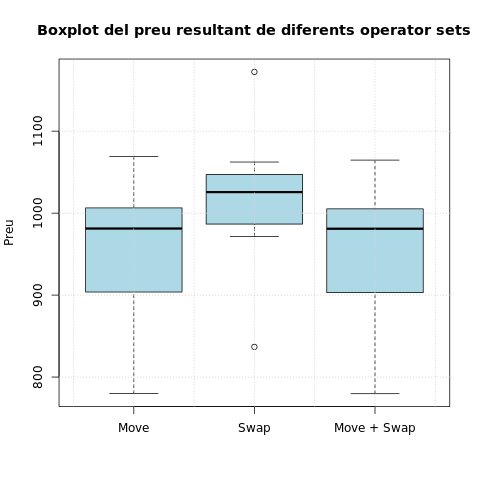
\includegraphics[width=0.45\textwidth]{images/exp1_boxplot.png}
		\caption{Boxplot del preu resultant de diferents operator sets}
		\label{fig:exp1_boxplot}
	\end{figure}
	
	\begin{table}[H]
		\centering
		\begin{tabular}{|c|c|c|c|c|}
			\hline
			\textbf{Operador} & \textbf{Mediana} & \textbf{Q1} & \textbf{Q3} & \textbf{IQR} \\
			\hline
			Move & 981.245 & 917.275 & 1003.02 & 85.745 \\
			\hline
			Swap & 1025.675 & 992.235 & 1046.285 & 54.05 \\
			\hline
			Move + Swap & 980.87 & 916.525 & 1002.11 & 85.5875\\
			\hline
		\end{tabular}
		\caption{Estadístiques del preu de diferents operator sets}
		\label{tab:exp1_estadisticas}
	\end{table}
	
	Com podem observar en la \textit{Figura \ref{fig:exp1_boxplot}}, el resultat obtingut amb l'operador \textit{swap} dista molt dels altres. Així que serà el primer que comentarem. Per començar, cal entendre que amb només un \textit{swap} no recorrerem tot l'espai de cerca per un simple motiu: una oferta de transport que inicialment tingui un paquet assignat mai més podrà estar buida. Aquesta limitació es reflecteix en una mediana major. Podem consultar les dades numèriques de l'experiment a la \textit{Taula \ref{tab:exp1_estadisticas}}. A més, veiem que el rang interquantílic (IQR) amb \textit{swap} és el menor, la qual cosa indica que aquest operador ens proporciona resultats consistents, però no els millors. \\
	
	Per altra banda, observem que els resultats de \textit{move} i \textit{move + swap} són molt similars. Això implica que amb el \textit{move} podem explorar la gran majoria de l'espai de cerca, ja que no té la restricció que presenta l'altre operador. En aquest cas, la única limitació que tindríem es donaria quan volguéssim fer un swap de dos paquets. Amb l'operador de \textit{move}, aquest procés s'ha de realitzar en dues operacions com a norma general; però, si un dels paquets no hi càpiga en l'altra oferta, necessitarem tres operacions, utilitzant una oferta auxiliar per assignar temporalment aquell paquet. \\
	
	En casos puntuals, seria probable que no poguéssim fer aquest swap només amb el \textit{move}. Aquest escenari s'ha donat durant els experiments, ja que en alguns casos hem observat una diferència molt petita en el cost, ja que el \textit{swap} ha pogut complementar el que el \textit{move} no podia. Per aquesta raó, els dos conjunts d'operadors que estem analitzant presenten resultats similars, però el conjunt que inclou l'operador \textit{swap} obté resultats lleugerament millors en alguns casos. \\
	
	Respecte a la nostra hipòtesi inicial, observem que s'ha complert, ja que el conjunt d'operadors que inclou tant \textit{move} com \textit{swap} ha mostrat un rendiment lleugerament superior en alguns casos. No obstant això, no esperàvem una similitud tan notable entre els resultats obtinguts amb els conjunts d'operadors $C_{\texttt{2}}$ i $C_{\texttt{3}}$. Aquesta similitud indica que l'operador \textit{swap} pot no ser essencial per millorar significativament els resultats en la majoria dels escenaris analitzats. \\
	
	A partir d'aquesta observació, podríem considerar l'opció de reduir el factor de ramificació eliminant l'operador \textit{swap} del conjunt d'operadors utilitzats. La raó darrere d'aquesta decisió es fonamenta en el principi d'eficiència: simplificar el conjunt d'operadors pot conduir a una reducció del temps de càlcul i a una millora en la velocitat d'exploració de l'espai de cerca. \\
	
	En resum, els resultats indiquen que, tot i que el \textit{swap} aporta certes millores en situacions particulars, la seva presència no és extremadament rellevant. Això suggereix que una aproximació més eficient podria ser treballar exclusivament amb l'operador \textit{move}, permetent-nos explorar l'espai de cerca de manera més àgil i reduint potencialment el factor de ramificació, facilitant així la millora del rendiment global de l'algoritme. \\
	
	
	\subsection{Experiment 2}
	
	Un altre punt que creiem molt important a l'hora de plantejar aquests problemes és la solució inicial. Una solució inicial de qualitat proporciona un diferent punt de partida per explorar l'espai de solucions, la qual cosa pot conduir a diferents resultats finals, o bé a una diferent velocitat per trobar una solució òptima. \\
	
	En aquest experiment, compararem dues estratègies de generació de solucions inicials per avaluar si hi ha alguna diferència notable en els resultats finals quan es fa servir l'algoritme \textit{Hill Climbing} i els operadors escollits a l'apartat anterior: \textit{swap} i \textit{move}.\\
	
	Les dues estratègies que considerarem per la generació de l'estat inicial són:
	
	\begin{itemize}
		\item \emph{Solució Inicial 2}: aquesta és una estratègia que genera solucions inicials amb una qualitat més alta, és a dir, busquem des d'un principi una solució més propera a la que creiem la solució final, més òptima, ja que intentem fer una assignació de paquets a ofertes amb el menor preu possible.
		
		\item \emph{Solució Inicial 2}: aquesta estratègia simplement pretén assignar els paquets a ofertes i en cap moment dona prioritat a les ofertes més barates, és per això que està més lluny de la solució final que busquem, però és més ràpia i simple de generar que la primera.
	\end{itemize}
	
	
	\begin{table}[ht]
		\centering
		\begin{tabular}{|l|p{10cm}|}
			\hline
			Plantejament & Observem la influència de dues solucions inicials en la qualitat de la solució final. \\
			\hline
			Hipòtesi & Una solució inicial menys òptima, la \textit{Solució inicial 2}, proporcionarà significativament millors resultats.\\
			\hline
			Mètode & 
			\begin{itemize}
				\item Agafarem un conjunt de $10$ llavors aleatòries.
				\item Establirem els algoritmes \textit{Hill Climbing} per un problema amb 100 paquets i una proporció de pes transportable per les ofertes d'1,2.
				\item Executarem els 10 experiments amb la \textit{Solució inicial 1} i la \textit{Solució inicial 2}, un per cada llavor.
				\item Medirem els resultats i n'extraurem conclusions.
			\end{itemize} \\
			\hline
		\end{tabular}
		\label{tab:exp2_apartats}
	\end{table}
	
	Els resultats, que es poden trobar al path \texttt{./Latex/spreadsheets/ex2.csv} de \textit{GitHub} (vegeu l'annex per accedir-hi), es poden resumir amb el gràfic i la taula que hi ha a continuació:
	
	\begin{figure}[H]
		\centering
		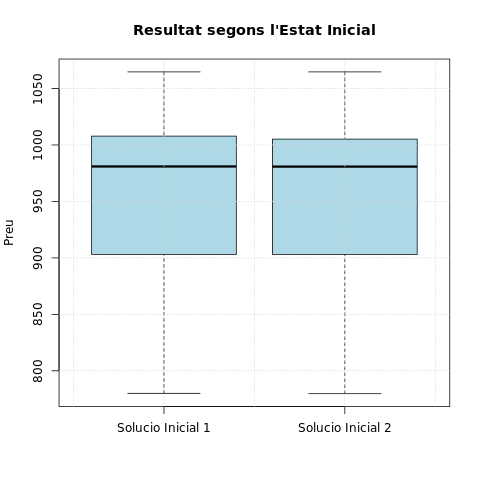
\includegraphics[width=0.45\textwidth]{images/exp2_boxplot.png}
		\caption{Boxplot del preu resultant segons la solució inicial}
		\label{fig:exp2_boxplot}
	\end{figure}
	
	\begin{table}[H]
		\centering
		\begin{tabular}{|c|c|c|c|c|}
			\hline
			\textbf{Operador} & \textbf{Mediana} & \textbf{Q1} & \textbf{Q3} & \textbf{IQR} \\
			\hline
			Solució 1 & 980.975 & 916.58 & 1004.178 & 87.5975 \\
			\hline
			Solució 2 & 980.87 & 916.525 & 1002.112 & 85.5875 \\
			\hline
		\end{tabular}
		\caption{Estadístiques del preu segons la solució inicial}
		\label{tab:exp2_estadisticas}
	\end{table}
	
	Com clarament veiem a la \textit{Figura \ref{fig:exp2_boxplot}}, les diferències entre els resultats obtinguts segons les solucions inicials donades són mínimes, tant en la mediana com en el rang interquartílic (IQR). La \textit{Solució inicial 1}, és a dir, la més "òptima", presenta una mediana respecte al preu lleugerament superior (980,975 comparada amb 980,87), però la diferència no és significativa. El rang interquartílic és també lleugerament més ampli per aquesta solució, amb un IQR de 87,60 en comparació amb els 85,59 de l'altra solució inicial.\\
	
	Aquestes similituds porten a pensar que ambdues estratègies acaben atrapades en mínims locals, independentment de la qualitat de la solució inicial, per això les diferències en els resultats finals són gairebé inexistents en l'algoritme de \textit{Hill Climbing}, és a dir, totes dues estratègies portaran cap a resultats similars.\\
	
	\textit{Conclusió} \\
	Després d'analitzar els resultats, podem concloure que no hi ha una diferència significativa entre les dues estratègies de generació de solucions inicials. Això ens dona a pensar que almenys en aquest escenari, l'algoritme \textit{Hill Climbing} tendeix a quedar-se en mínims locals, independentment de la qualitat de la solució inicial. Per tant, pels pròxims experiments, optarem per la generació de solucions inicials menys òptimes, és a dir, per la \textit{Solució inicial 2}, ja que simplifica el procés de generar l'Estat Inicial i no empitjora la solució final.\\
	
	\subsection{Experiment 3}
	
	\newpage
	\section{Conclusions}
	
	
	\newpage
	\section{Treball d'Innovació: DeepVariant}
	
	\subsection{Tema}
	Hem escollit DeepVariant, un algorisme de machine learning desenvolupat per Google, que utilitza xarxes neuronals profundes per identificar variants genètiques en dades de seqüenciació de l'ADN. Mitjançant imatges generades a partir de les lectures de seqüència, DeepVariant detecta mutacions petites amb una precisió superior respecte a altres mètodes tradicionals.
	
	\subsection{Responsabilitats d'equip}
		Malgrat que el treball s'està fent col·laborativament i tots els membres del grup participen en totes les tasques, s'ha decidit dividir-ho en tres parts per cercar i aconseguir informació al respecte.
	\begin{itemize}
		\item \emph{Introducció i context}:\\
			Introducció a DeepVariant: què és i per què és rellevant.\\
			Importància de DeepVariant en la detecció de variants genètiques.\\
			Visió general del problema que resol en l'anàlisi de dades de seqüenciació d'ADN.\\
			Per què l'aprenentatge profund és útil en aquest context: beneficis respecte als mètodes tradicionals de detecció de variants (comparació amb altres mètodes).\\
			
		\item \emph{Xarxes Neuronals Convolucionals (CNN)}:\\
			Explicació de què són les xarxes neuronals convolucionals (CNNs).\\
			Com s'utilitzen les CNNs en DeepVariant per identificar patrons genètics.\\
			Avantatges de l'ús de CNNs per analitzar dades de seqüenciació d'ADN (perquè reconeixen patrons visuals).\\
			Relació entre les imatges generades per DeepVariant i l'anàlisi de dades genètiques.\\
			
		\item \emph{Funcionament Pipeline}:\\
			Generació d'imatges a partir de dades de seqüenciació d'ADN.\\
			Com les imatges es passen per la xarxa neuronal convolucional per ser classificades.\\
			Processos d'inferència: com es decideix quina variant està present (substitució, inserció, deleció).\\
			Entrenament de la xarxa neuronal amb dades genètiques.\\
			Presa de decisions sobre la presència de variants genètiques i avantatges de precisió i fiabilitat.\\
	\end{itemize}
	
	
	
	\subsection{Fonts}
	\begin{itemize}
		\item \emph{Creating a universal SNP and small indel variant caller with deep neural networks}:
		Rellevància: Base teòrica de DeepVariant i explicació de l'ús de xarxes neuronales.
		Data d'accés: 13 d'octubre de 2024
		Enllaç: https://doi.org/10.1101/092890
		***********SEGONA PART AL WHATS
		\item \emph{}:
		Enllaç: https://github.com/google/deepvariant
		També porta a altres documents com: https://google.github.io/deepvariant/posts/2020-02-20-looking-through-deepvariants-eyes/
	\end{itemize}
	
	\subsection{Dificultats}
	\begin{itemize}
		\item \emph{Accés a referències}: Alguns articles rellevants requereixen subscripcions per poder obtenir informació detallada.
		\item \emph{Informació tècnica}: Hem hagut de fer un sobreesforç perquè es requereix d'un mínim de coneixements sobre l'ADN per entendre la proposta.
	\end{itemize}

	
	
	

\end{document}